	\chapter{Monte--Carlo--Integration}\label{chapter:mc_integration}
	Monte--Carlo--Verfahren liegt die Idee zugrunde, zu einem numerischen Problem ein passendes Zufallsexperiment so zu konstruieren, so dass der Erwartungswert einer Zufallsvariable des Experiments das numerische Problem l"ost.
	
	Die Idee ist nicht neu, so f"uhrte {\em Buffon} 1777 folgendes Experiment durch: Eine Nadel der L"ange $L$ wird wiederholt auf eine plane Fl"ache mit parallelen Linien im Abstand $d>L$ fallengelassen und jeweils notiert, ob die Nadel eine der Linien kreuzt. Er zeigte, dass der Erwartungswert f"ur die Wahrscheinlichkeit der Nadel, die Linie zu kreuzen $$p=\frac{2L}{\pi d}$$ betr"agt. Laplace wies sp"ater darauf hin, dass  man die H"aufigkeit, mit der die Nadeln die Linien kreuzen, auch Nutzen kann, um den Wert von $\pi$ zu sch"atzen (siehe Abb. \ref{fig:buffon}): $$\pi=\frac{2L}{p d}\approx \frac{2L}{\frac{k}{N}d}$$
	(\text{N Experimente, davon k mal eine Linie gekreuzt}).
	\begin{figure}
		\centering
		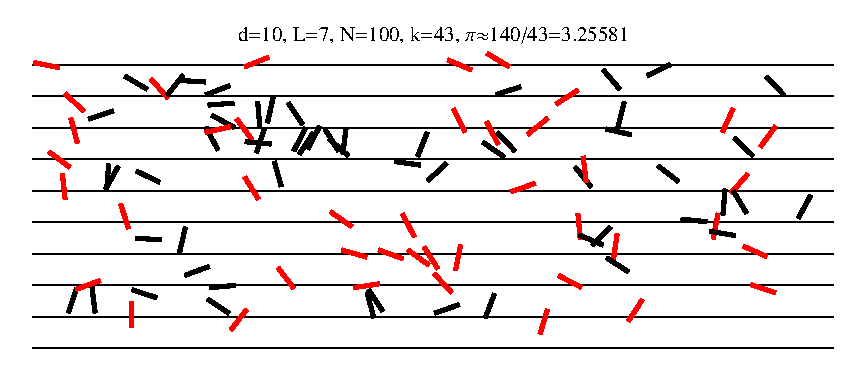
\includegraphics[height=0.3\textheight]{buffonsneedles.eps}
		\caption{Beispiel f"ur eine Realisierung des Buffon--Nadel--Experiments mit 100 geworfenen Nadeln. Der erhaltene Sch"atzwert f"ur $\pi$ ist bei so wenigen Nadeln nicht sehr genau.}
		\label{fig:buffon}
	\end{figure}
	
	\section{Das Integrationsproblem}\label{subsec:integrationsproblem}
	Betrachten wir das Integral
	\begin{equation}
		I=\int_\Omega f(x) d\mu(x),
		\label{eq:integration_problem}
	\end{equation}
	wobei $\Omega$ das Integrationsgebiet, $f : \Omega \to \mathbb{R}$ eine reellwertige Funktion und $\mu$ ein Ma"s auf $\Omega$ ist. F"ur die folgende Darstellung nehmen wir an, dass $$\Omega=[0,1]^d$$ der $d$--dimensionale Einheitsw"urfel und $I_d$ das zugeh"orige Integral ist.
	\subsection{Klassische numerische Quadraturverfahren}
	Die klassische numerische Herangehensweise (wenn keine analytische L"osung m"oglich oder praktikabel ist) sind {\em Tensor--Produkt--Verfahren}. Die Idee dabei ist, f"ur jede Dimension ein eindimensionales Quadratur--Verfahren zu w"ahlen (verschiedene oder das gleiche) und diese zu einem mehrdimensionalen Verfahren zu kombinieren. Ein eindimensionales Verfahren stellt eine gewichtete Summe von Funktionswerten an $M$ (vor dem Auswerten der Funktion) festgelegten St"utzstellen dar:
	$${\tilde I}_1=\sum_{i=1}^M w_i\,f(x_i).$$
	Bekannte Vertreter dieser eindimensionalen Quadraturregeln sind z.B. die {\em Newton--Cotes}- und {\em Gauss--Legendre}--Verfahren. Ein hieraus konstruiertes Tensor--Produkt--Verfahren (wobei wir der Einfachheit halber f"ur alle Dimensionen dasselbe eindimensionale Verfahren zugrundelegen) hat dann die Form:
	$${\tilde I}_d^{\,\text{TP}}=\sum_{i_1}^M\cdots\sum_{i_d}^M w_{i_1}w_{i_2}\cdots w_{i_d}f(x_{i_1},\cdots,x_{i_d}).$$
	Aus einem eindimensionalen Verfahren mit $M$ St"utzstellen erhalten wir also ein $d$--dimensionales Verfahren mit $M^d$ St"utzstellen (Siehe Abb. {\ref{fig:tensorproduct}}).
	\begin{figure}
		\centering
		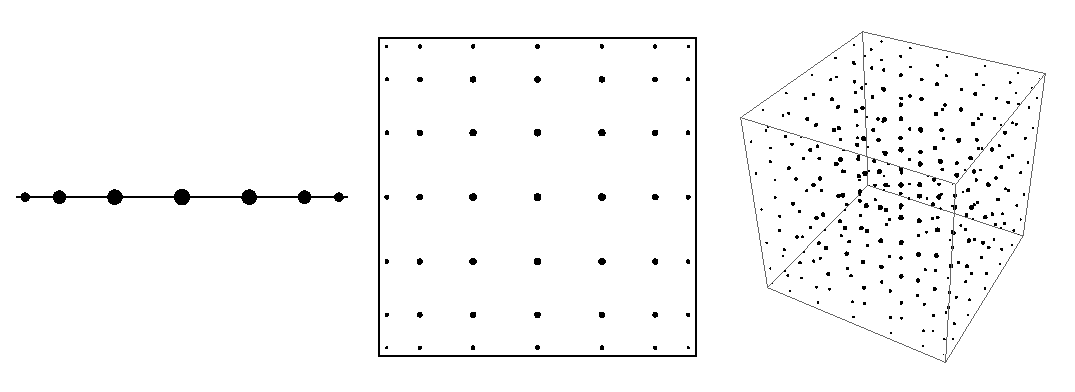
\includegraphics[height=0.25\textheight]{tensorproduct_quadrature.eps}
		\caption{St"utzstellen eines 1D 7--Punkt--Gauss--Legendre--Verfahrens und entsprechender Tensor--Produkt--Verfahren f"ur 2 bzw. 3 Dimensionen. Die Gewichte der St"utzstellen sind durch ihre Gr"o"se kenntlich gemacht.}
		\label{fig:tensorproduct}
	\end{figure}
	
	\subsection{einfache Monte--Carlo--Integration}
	Bei der Monte--Carlo--Integration ziehen wir $N$ zuf"allige, gem"a"s einer Wahrscheinlichkeitsdichte $p$ verteilte St"utzstellen $[X_i|i\in\{1,\dots,N\}]$ in $\Omega$ und sch"atzen dann den Wert des Integrals (\ref{eq:integration_problem}) mit
	\begin{equation}
		{\tilde I}_d^{\,\text{MC}}=\frac{1}{N}\sum_{i=0}^{N-1} \frac{f(X_i)}{p(X_i)}
		\label{eq:mc_integral}
	\end{equation}
	ab. Im Falle unseres $d$--dimensionalen Einheitsw"urfels $\Omega=[0,1]^d$ k"onnen wir besipielsweise jede St"utzstelle aus $d$ gleichf"ormig auf dem Einheitsintervall $[0,1]$ verteilten Zufallszahlen $U_i$ durch einfache Tupelbildung
	$$X_i:=(U_{d i},\dots,U_{d(i+1)-1})$$
	gewinnen. Aber auch f"ur allgemeine Integrationsgebiete $\Omega$ kann das Verfahren genauso angewandt werden, solange ein passendes Integrationsma"s $\mu$ und ein Wahrscheinlichkeitsma"s $P$ existieren, so dass $$P(D)=\text{Pr}(x\in D)$$ f"ur jede me"sbare Menge $D\subset\Omega$ gilt. Die entsprechende Wahrscheinlichkeitsdichte $p$ l"asst sich mit Hilfe der {\em Radon--Nikodym--Ableitung} $$p(x)=\frac{dP}{d\mu}(x)$$
	einf"uhren, wobei $p$ dann einfach eine Funktion ist, f"ur die $$P(D)=\int_D p(x)d\mu(x)$$ gilt.
	Von der Erwartungstreue des Sch"atzers (\ref{eq:mc_integral}) f"ur unser Integral (\ref{eq:integration_problem}) k"onnen wir uns mit \citep[][2.4]{Veach:1997p9136}
	\begin{align*}
		E[{\tilde I}_d^{\,\text{MC}}] &=E\left[\frac{1}{N}\sum_{i=0}^{N-1}\frac{f(X_i)}{p(X_i)}\right] \\
			&= \frac{1}{N}\sum_{i=0}^{N-1}E\left[\frac{f(X_i)}{p(X_i)}\right] \\
			&= \frac{1}{N}\sum_{i=0}^{N-1}\int_\Omega \frac{f(X_i)}{p(X_i)}p(X_i)\,d\mu(x) \\
			&= \int_\Omega f(x)\,d\mu(x)\\
			&= I
	\end{align*}
	leicht "uberzeugen.
	
	\subsection{Konvergenzraten}\label{subsec:integrationsproblem_comparison}
	Wir wollen nun die Konvergenzraten der Tensor--Produkt--Verfahren mit der Konvergenzrate des einfachen Monte--Carlo--Sch"atzers (\ref{eq:mc_integral}) vergleichen. Zur Konstruktion eines Vertreters der Tensor--Produkt--Verfahren verwenden wir beispielhaft das Newton--Cotes--Verfahren. In \citep[][3.1.4]{Stoer:2005p10586} wird als Ab\-sch"at\-zung f"ur den Fehler eines Verfahrens $p$--ter Ordnung (d.h. ein Verfahren, das alle Polynome bis zum Grad $p$ exakt integriert) und Schrittweite $h(\approx\frac{b-a}{N}=\mathcal{O}(N^{-1}))$ der St"utzstellen
	\begin{equation}
		\int_a^b P_n(x)-f(x)dx=h^{p+1}K f^{(p)}(\xi),\quad\xi\in(a,b)
		\label{eq:quadrature_error}
	\end{equation}
	angegeben, wobei $n$ die Anzahl der St"utzstellen, $P_n$ das Interpolationspolynom f"ur die St"utzstellen und K eine Konstante ist. Gauss--Legendre--Verfahren sind von der Ordnung $2n-1$, d.h. die Konvergenzrate dieser $n$--Punkt--Formel ist demnach von der Gr"o"senordnung $\mathcal{O}(h^{2n})=\mathcal{O}(N^{-2n})$.\footnote{$N$ bezeichnet die Anzahl der St"utzstellen f"ur das gesamte Integrationsintervall. Der Sch"atzwert f"ur das Integral wird dann durch $\frac{N}{n}$--maliges Anwenden der $n$--Punkt--Formel berechnet}
	Durch Bildund der entsprechenden $d$--dimensionalen Tensor--Produkt--Regel "andert sich die Konvergenzrate in Bezug auf die Schrittweite $h$ nicht. Da unsere $N$ St"utzstellen sich nun aber auf ein $d$--dimensionales Gitter verteilen, teilt sich das Volumen unseres $d$--dimensionalen Einheitsw"urfels in $N$ W"urfel mit einem Volumen von jeweils $h^d$ auf, d.h. f"ur die Schrittweite folgt
	$$\mathcal{O}(1)=V=N h^d \Rightarrow h=\mathcal{O}\left(\left(\frac{1}{N}\right)^{1/d}\right)=\mathcal{O}\left(N^{-1/d}\right)$$	
	und damit f"ur die Konvergenzrate in Bezug auf die Gesamtst"utzstellenzahl
	$$\mathcal{O}(h^{2n})=\mathcal{O}(N^{-2n/d}).$$
	Dies bedeutet, dass Tensor--Produktverfahren mit steigender Dimension des Integrationsgebietes an Effizienz verlieren. Bei hochdimensionalen Problemen kann dies kaum durch Verfahren h"oherer Ordnung ausgeglichen werden, da Verfahren h"oherer Ordnung, wie oben in (\ref{eq:quadrature_error}) zu sehen auch gr"o"sere Anforderungen an die Glattheit der Funktion stellen. Ausserdem kann die exponentiell steigende Anzahl aller $N \geq n^d$ mindestens n"otigen Funktionsaufrufe zu einem Problem werden. Der Effekt wird bei steigender Dimension und Ordnung des Verfahrens nur noch schlimmer, was ein Ausgleichen der schlechteren Konvergenzrate bei h"oheren Dimensionen durch Erh"ohen der Ordnung des Verfahrens schnell praktisch unm"oglich werden l"asst. Dies wird h"aufig als {\em Curse~of~Dimensionality} (Fluch der Dimensionalit"at) bezeichnet.
	
	Bei der Monte--Carlo--Integration k"onnen wir die Konvergenzrate anhand der Varianz unseres Monte--Carlo--Sch"atzers (\ref{eq:mc_integral}) bestimmen \citep[][2.4.1]{Veach:1997p9136}. Nennen wir der "Ubersicht wegen
	$$Y_i=\frac{f(X_i)}{p(X_i)}$$
	und den MC--Sch"atzer mit $N$ gezogenenen Werten
	$$F_N=\frac{1}{N}\sum_{i=0}^{N-1} Y_i.$$
	Dann gilt f"ur die Varianz eines beliebigen Samples
	\begin{equation}
		V[Y_i]=E[(Y_i-E[Y_i])^2]=E[Y_i^2]-E[Y_i]^2=\int_\Omega \frac{f(x)^2}{p(x)}d\mu(x)-I^2.
		\label{eq:mc_variance}
	\end{equation}
	Da die Werte unabh"angig gezogen sind gilt f"ur die Varianz des Sch"atzer mit $N$ Werten
	$$V[F_N]=V\left[\frac{1}{N}\sum_{i=0}^{N-1}Y_i\right]=\frac{1}{N^2}V\left[\sum_{i=0}^{N-1}Y_i\right]=\frac{1}{N^2}\sum_{i=0}^{N-1}V[Y_i]=\frac{1}{N}V[Y_i],$$
	d.h. die Varianz des Sch"atzers sinkt invers mit der Anzahl $N$ an gezogenen Werten. Daraus folgt sofort die Standardabweichung
	\begin{equation}
		\sigma[F_N]=\frac{1}{\sqrt{N}}\sigma[Y_i],
		\label{eq:mc_standarddeviation}
	\end{equation}
	was einer Konvergenzrate von $\mathcal{O}(N^{-1/2})$ entspricht. Die Konvergenzrate des Monte--Carlo--Sch"atzers ist im Gegensatz zur Konvergenzrate der Tensor--Produkt--Verfahren also unabh"angig von der Dimension des Integrationsgebietes, d.h. das Verfahren leidet {\em nicht} unter dem {\em Curse~of~Dimensionality}! Ausserdem mussten wir nirgendwo Bedingungen an die Glattheit der Funktion stellen, was bei Funktionen mit Diskontinuit"aten von Vorteil ist.
	
	Zusammenfassend k"onnen wir also feststellen, dass Monte--Carlo--Integration bei hochdimensionalen Integrationsproblemen und Funktionen mit Diskontinuit"aten klar gegen"uber klassischen Tensor--Produktverfahren vorzuziehen ist. F"ur niedrigdimensionale ($d\lessapprox 7$) Gebiete mit glatten Integranden sind die klassischen Methoden hingegen besser geeignet.
	
	
	\section{Importance--Sampling}\label{subsec:importancesampling}
	Wir sind bei unserem MC--Sch"atzer (\ref{eq:mc_integral}) nicht darauf beschr"ankt eine gleich\-f"or\-mi\-ge Wahrscheinlichkeitsdichte $p$ zu w"ahlen. Es kann die Effizienz des Verfahrens sogar betr"achtlich verbessern, wenn wir eine geeignete Wahrscheinlichkeitsdichte $p$ w"ahlen. Schauen wir uns daher die Formel (\ref{eq:mc_variance}) f"ur die Varianz, die es zu minimieren gilt, nochmal an, um zu verstehen, was ``geeignet'' bedeutet. Nimmt die Wahrscheinlichkeitsdichte beispielsweise die ideale Form
	\begin{equation}
		p(x)=\frac{|f(x)|}{\int_\Omega |f(z)|d\mu(z)}
		\label{eq:ideal_importance_pdf}
	\end{equation}
	an, kann man mit der {\em Jensenschen~Ungleichung} zeigen, dass dann das Integral in (\ref{eq:mc_variance}) und damit die Varianz insgesamt minimal wird. Nimmt $f$ keine negativen Werte an, verschwindet die Varianz dieses Sch"atzers sogar, da in (\ref{eq:mc_integral}) dann nur noch "uber die konstante L"osung (in Form der Normierungskonstanten) gemittelt wird. Wenn wir das Normierungs--Integral im Nenner von (\ref{eq:ideal_importance_pdf}) l"osen k"onnten, w"are allerdings auch die urspr"ungliche Integration (\ref{eq:integration_problem}) kein Problem! Daher suchen wir in der Praxis nach einem $p$, das m"oglichst "ahnlich zu $|f|$ und gleichzeitig normierbar ist.
	
